\chapter{Methodology}

To apply the previously mentioned balancing methods to Cal Poly's SADS, significant progress was made on it's design both at the software and hardware level. Namely, a closed-loop feedback system was designed including a measurement system for attitude determination, a flight computer to process measurements and generate commands in real time, and linear actuators to shift the platform's center of mass.

\section{System Architecture}

\begin{figure}
    \centering
    \usetikzlibrary{arrows.meta,positioning,fit,calc,shapes.misc}
\usetikzlibrary{shapes.geometric,quotes}

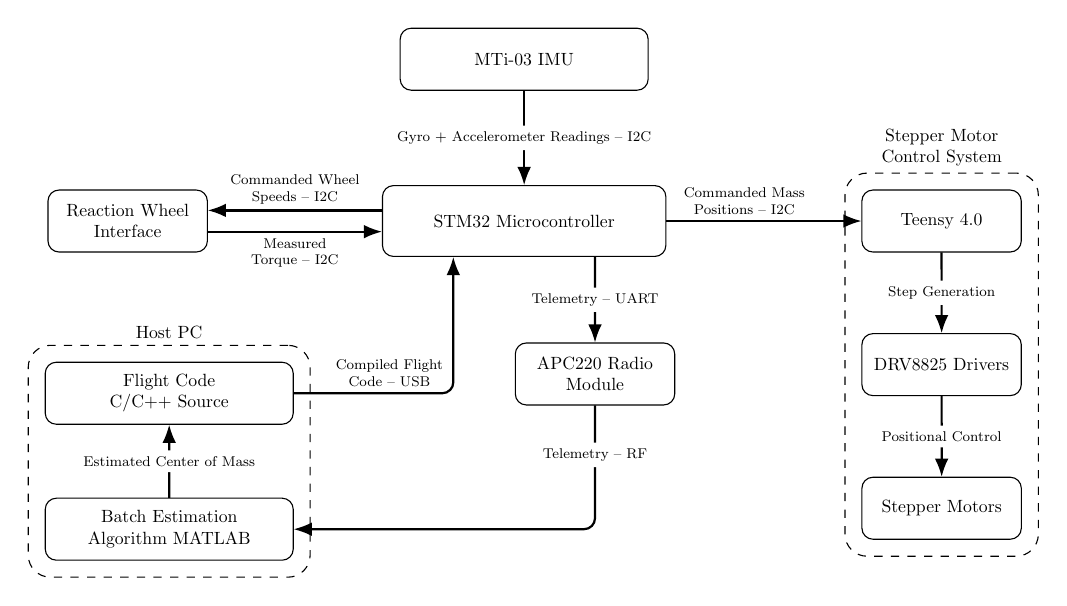
\begin{tikzpicture}[
  scale=0.64,
  every node/.style={transform shape},
  line/.style={draw, -Latex, thick, rounded corners=4pt},
  box/.style={rectangle, draw, rounded corners, align=center, fill=white,
              minimum width=16em, minimum height=4em},
  smallbox/.style={rectangle, draw, rounded corners, align=center, fill=white,
              minimum width=14em, minimum height=3.5em},
  extbox/.style={rectangle, draw, dashed, rounded corners=8pt, inner sep=6pt}
]

% =======================================================
%                     MAIN COMPONENTS
% =======================================================
\node[box] (stm32) at (0,0) {STM32 Microcontroller};
\node[smallbox] (mti) [above=of stm32, yshift=2.5em] {MTi-03 IMU};

\coordinate (telem_out) at ($(stm32.south)+(4em,0em)$);
\coordinate (fc_in) at ($(stm32.south)+(-4em,0em)$);
\node[smallbox,minimum width=9em] (apc) [below=of telem_out, yshift=-2em] {APC220 Radio\\Module};
\node[smallbox,minimum width=9em] (rwi) [left=of stm32, xshift=-7em] {Reaction Wheel\\Interface};

% Teensy subsystem (right side)

\node[smallbox,minimum width=9em,right = of stm32,xshift=19ex] (teensy)  {Teensy 4.0};
\node[smallbox,minimum width=9em,below = of teensy,yshift=-4ex] (drv) {DRV8825 Drivers};
\node[smallbox,minimum width=9em,below = of drv,yshift=-4ex] (steppers) {Stepper Motors};

% Host PC subsystem (left bottom)

\node[smallbox,below left=of stm32,xshift=-5ex,yshift=-25ex] (matlab) {Batch Estimation\\ Algorithm MATLAB};
\node[smallbox, above = of matlab,yshift=3ex] (fc)  {Flight Code\\C/C++ Source};
% =======================================================
%                     CONNECTIONS
% =======================================================

% IMU → STM32
\draw[line] (mti.south) -- 
node[fill=white, font=\footnotesize]  {Gyro + Accelerometer Readings -- I2C}
(stm32.north);

% Reaction Wheel Interface ↔ STM32
\coordinate (wheel_out) at ($(stm32.west)+(0em,0.6em)$);
\coordinate (torque_in) at ($(stm32.west)+(0em,-0.6em)$);
\draw[line] (wheel_out) --  
  node[above, font=\footnotesize,align=center, text width=20ex] {Commanded Wheel Speeds -- I2C} 
($( rwi.east |- wheel_out)$) ;
\draw[line] ($( rwi.east |- torque_in)$) --
  node[below, font=\footnotesize,align=center, text width=20ex] {Measured Torque -- I2C} (torque_in);

% STM32 → Teensy (Commanded Mass Positions)
\draw[line] (stm32.east) -- 
  node[above, font=\footnotesize, pos=0.4,align=center,text width = 17ex] {Commanded Mass Positions -- I2C} 
(teensy.west);

% Teensy downward chain
\draw[line] (teensy.south) -- node[fill=white, font=\footnotesize]
  {Step Generation} (drv.north);
\draw[line] (drv.south) -- node[fill=white, font=\footnotesize]
  {Positional Control} (steppers.north);

% Host PC internal (Simulink → Flight Code)
\draw[line] (matlab.north) -- 
  node[fill=white, font=\footnotesize] {Estimated Center of Mass} 
(fc.south);

% Host PC → STM32 (USB upload)
\draw[line] (fc.east) -|
  node[align=center, text width=15ex,above, font=\footnotesize, pos=0.3] {Compiled Flight\\Code -- USB} 
(fc_in);

% STM32 → APC220 (UART telemetry)
\draw[line] (telem_out) -- 
    node[font=\footnotesize,fill=white] {Telemetry -- UART} 
(apc.north);

% Telemetry RF (Host PC → APC)
% \coordinate (rfbus) at ($(stm32.south)+(0,-4)$);
% \draw[line] (matlab.east) -- node[above, font=\footnotesize]
%   {Telemetry -- RF} (rfbus -| matlab.east) -- (rfbus -| apc.south);
% \draw[line] (rfbus -| apc.south) -- (apc.south);
\draw[line] (apc.south) |- 
    node[fill=white,pos=0.2,font=\footnotesize]{Telemetry -- RF}
(matlab.east);

\node[extbox, fit=(fc)(matlab), label={[align=center]above:Host PC}] (host) {};
\node[extbox, fit={(teensy)(drv)(steppers)}, label={[align=center]above:Stepper Motor\\Control System}] (teensybox) {};

\end{tikzpicture}
    \caption{Operation flowchart during passive balancing}
    \label{fig:sys_arch_passive}
\end{figure}

\begin{figure}
    \centering
    \input{figures/sys_arch_active.tikz}
    \caption{Operation flowchart during active balancing}
    \label{fig:sys_arch_active}
\end{figure}


\section{Mechanical}

The goal of the mechanical design was to build off work completed in \cite{gilman_automatic_2024} and develop set of low-cost linear actuators that finely control the position of mass blocks. Taking lessons learned from previous iterations, the second main goal was to ensure that the size of the mass blocks was highly customizable, thus making the resulting center of mass envelope customizable. 

\subsection{Mass Sizing}

While the exact final design and mass properties of the SADS is unknown, it is still important to place an approximate upper bound on the size of the mass blocks driven by the linear actuators. This ensures that the motors and mounting hardware are not oversized and do not excessively increase the simulator's moment of inertia. A common metric used to help quantify this is a simulator's center of mass envelope. This is the set of all values $\Delta\mathbf{r}$ that the system can command when all linear actuators are in their centered positions.

One important aspect of the SADS when selecting it's desired center of mass envelope is it's symmetrical design. The two heaviest systems onboard are the reaction wheels and the mass balancing system itself. The pyrimdal reaction wheel configuration means the wheels contribute little horizontal inbalance. and the wheels are roughly on the same horizontal plane as the platform's center of rotation, so they also contribute little verical inbalance. The linear actuator design will follow the same general layout in \cite{gilman_automatic_2024}, which can be seen in FIGURE. 

The main source of inbalance will thus be introduced by relatively lighter components like batteries, sensors, the flight computer, and other miscellaneous electronics. To approximate a worse case inbalance, the heaviest of these components - the main 24V battery was placed in CAD in multiple unfavorable positions with the resulting inbalance vector recorded. 

% Isometric + Top Down CAD view of Gilman's design

\subsection{Linear Actuator Design}

The linear actuators use the same mounting configuration as the previous design. A ball screw is fixed 

% images of the ball screw and plate solution + CAD?

\section{Electrical}

The primary goal of the electrical design is to interface the newly developed linear actuators and an IMU to the flight computer. An STM32F446RE was chosen as the primary flight computer. This board has high number of GPIO pins, a maximum clock speed of 180 MHz, is low cost, and has proven compatibility with Simulink hardware suppport packages, making it desirable for this project. Despite these benefits, using a microcontroller still has numerous drawbacks, the main one being the need to reflash the board to switch bewteen programs. In the final iteration of the SADS, the flight computer ideally runs as a Linux-based RTOS, where the operator can easily load and switch between multiple programs. 

An MTi-03 was chosen as the IMU REFERRING TO LITERATURE REVIEW for it's noise characteristics and easy of integration with the STM32. The primary electrical interface between the IMU and flight computer are the  



% electrical diagram 

\section{Software}

\begin{figure}
    \centering
    \usetikzlibrary{arrows.meta,positioning,fit,calc,shapes.misc}
\usetikzlibrary{shapes.geometric}

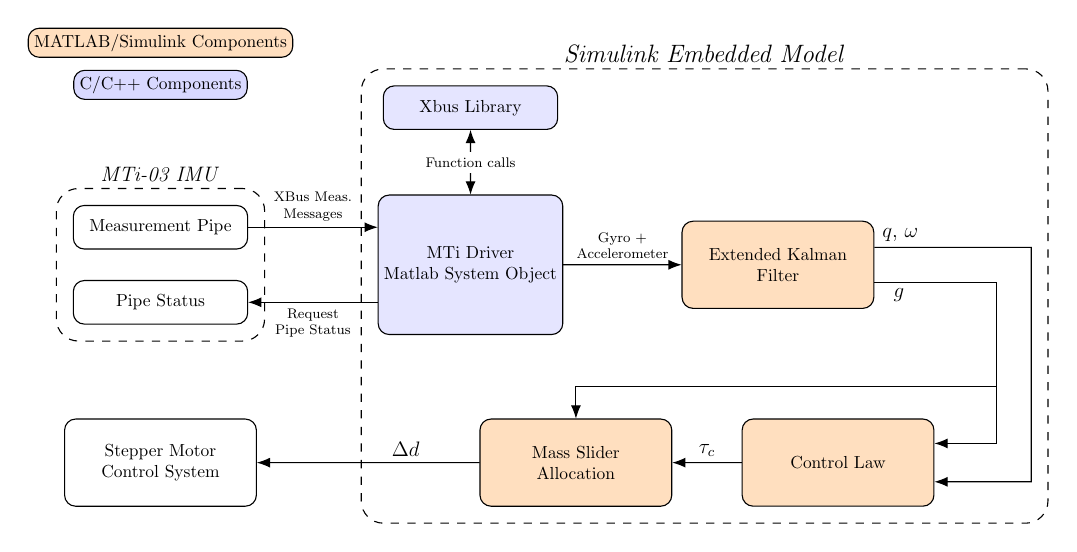
\begin{tikzpicture}[
    scale=0.63,                        % <-- change this to resize (e.g., 0.8 or 1.3)
    every node/.style={transform shape},
    node distance=2em and 4em,
    line/.style={-Latex},
    block/.style={
        rectangle, draw, rounded corners,
        fill=blue!15, align=center,
        minimum width=11em, minimum height=5em
    },
    smallblock/.style={
        rectangle, draw, rounded corners,
        fill=blue!10, align=center,
        minimum width=10em, minimum height=2.5em
    },
    tallblock/.style={
        rectangle, draw, rounded corners,
        fill=blue!10, align=center,
        minimum width=10em, minimum height=8em
    },
    extbox/.style={rectangle, draw, dashed, rounded corners=8pt, inner sep=6pt},
    callout/.style={font=\footnotesize, midway, fill=white, inner sep=1pt}
]

% -------------------- LEFT EXTERNAL (IMU) --------------------


\node[smallblock,  yshift=-5ex,fill=white]  (p_status) {Pipe Status};
\node[smallblock, yshift=5ex,fill=white]  (meas_pipe) {Measurement Pipe};
\node[extbox, fit=(p_status)(meas_pipe),label={[align=center]above:\large{\textit{MTi-03 IMU}}}] (imu) {}; 
% -------------------- MAIN SYSTEM --------------------
\node[tallblock, right=of p_status,xshift=8ex,yshift=5ex] (driver) {MTi Driver\\ Matlab System Object};
\node[smallblock, above=of driver, yshift=4ex] (xbus) {Xbus Library};
\node[block, right=of driver,xshift=6.5ex,fill=orange!25] (ekf) {Extended Kalman\\Filter};
\node[block, below=of ekf,xshift=8ex,yshift=-10ex,fill=orange!25] (ctrl) {Control Law};
\node[block, left=of ctrl,fill=orange!25] (alloc) {Mass Slider\\Allocation};

\node[block,fill=white] (stepper) at ($(p_status |- alloc)$){Stepper Motor\\ Control System};


% -------------------- CONNECTIONS --------------------
\draw[line] (meas_pipe.east) -- 
    node[above,font=\footnotesize, align=center, text width=15ex] {XBus Meas. Messages}
($(driver.west |- meas_pipe.east)$);

\draw[line] ($(driver.west |- p_status.east)$) -- 
    node[below,font=\footnotesize, align=center, text width=15ex] {Request Pipe Status}
(p_status.east);

\draw[line,Latex-Latex] (xbus) -- 
    node[fill=white,font=\footnotesize] {Function calls}
(driver);

\draw[line] (driver) -- 
    node[above,font=\footnotesize, align=center, text width=15ex] {Gyro +\\Accelerometer}
(ekf);

\coordinate (ekfOut1) at ($(ekf.east)+(0em,1em)$);
\coordinate (ekfWrap1) at ($(ekfOut1)+(9em,0)$);   % distance right; tweak 4em as you like

\coordinate (ekfOut2) at ($(ekf.east)+(0em,-1em)$);
\coordinate (ekfBranch) at ($(ekfOut2)+(7em,-6em)$);   % distance right; tweak 4em as you like

\draw[line] (ekfOut1) -- 
    node[above, align=center,xshift=-7ex,font=\large] {$\bm{q}$, $\bm{\omega}$}
(ekfWrap1) |- ($(ctrl.east)+(0,-1.1em)$);
\draw[line] (ekfOut2) -| 
    node[below,xshift=-13ex,font=\large] {$\bm{g}$}
(ekfBranch) |- ($(ctrl.east)+(0,+1.1em)$);
\draw[line] (ekfBranch) -| (alloc);
\draw[line] (ctrl) --
    node[above, align=center,font=\large] {$\bm{\tau}_c$}
(alloc);
\draw[line] (alloc) -- 
    node[above, align=center,xshift=5ex,font=\large] {$\Delta\bm{d}$} 
(stepper);

% Boundary box for Simulink model
\node[extbox, fit=(xbus)(driver)(ekf)(ctrl)(alloc)(ekfWrap1),
    label={[align=center]above:\Large{\textit{Simulink Embedded Model}}}] (simbox) {};

\node[draw, fill=orange!25, rounded corners,above=of meas_pipe,yshift=15ex] (sim) {MATLAB/Simulink Components};
\node[draw, fill=blue!15, below=of sim, rounded corners,yshift=3ex] (c) {C/C++ Components};

\end{tikzpicture}
    \caption{Functional software architecture during balancing}
    \label{fig:software_flowchart}
\end{figure}

% xbus flow chart - measurement system design

% software flow chart in config mode
% software flow chart in real time control


\section{Algorithm Implementation}

% real time Kalman filter with gravity vector?
% discussion of Simulink code generation - PID + adaptive control

% feedback control diagrams

% unscented Kalman filter detailed derivation